
\chapter[Darstellung der Grundlagen ]{Darstellung der Grundlagen} \label{Kapitel2}
\minitoc
\newpage
\section{SECONDO}\label{SecondoEinfuehrung}

\subsection{Einführung}
SECONDO ist ein erweiterbares Datenbank"-management-System (DBMS), das vom Lehrgebiet Praktische Informatik IV, ,,Datenbanksysteme für neue Anwendungen'', in der Fakultät Mathematik und Informatik der Fernuniversität Hagen entwickelt wurde und kontinuierlich weiterentwickelt wird.

Das Ziel von SECONDO ist es, ein ,,allgemeines'' Datenbanksystem--Framework zur Verfügung zu stellen, dass mit Implementierungen von verschiedenen DBMS--Datenmodellen gefüllt werden kann.

Mit diesem soll es möglich sein, relationale, objektorientierte, zeitliche oder XML-Modelle zu implementieren und Datentypen für räumliche Daten, bewegte Objekte, graphentheoretische Strukturen oder Schachspiele zu speiichern und Operationen darauf durchzuführen. Die Möglichkeit zur Änderung des grundlegenden Datenmodells ist eine Besonderheit von SECONDO. Für die Erweiterbarkeit des Systems sind die ,,SECONDO-Algebren'' zuständig, deren Konzept weiter unten näher beleuchtet wird.

Das SECONDO-System setzt sich im Wesentlichen aus drei Komponenten zusammen:
\begin{enumerate}
\item Der Kernel

Der Kernel ist für die Datenhaltung und für die Abfragebearbeitung in der speziellen SECONDO--Syntax zuständig. Datenpersistenz erreicht der Kernel durch das Zusammenspiel mit einer BerkleyDB. Die Algebren zur Unterstützung verschiedener Datentypen werden in den Kernel gelinkt. Der Kernel und die meisten Algebren sind in C++ geschrieben, es gibt aber auch die Möglichkeit, Algebren in Java zu kodieren.

\item Der Optimizer

Der Optimizer bietet die Möglichkeit, Datenbankanfragen in einer eigenen, SQL--ähnlichen Syntax zu formulieren. Der Optimizer findet für diese Abfragen eine optimale Ausführung, indem er etwa den besten Join--Typ einer Abfrage bestimmt oder die Reihenfolge der Abarbeitungen ändert. Der Optimizer ist in PROLOG geschrieben. Die vorliegende Arbeit verwendet die Möglichkeiten des Optimizers nicht.

\item Das GUI

Das SECONDO-GUI bietet eine komfortabele Möglichkeit, entweder direkt oder  über den Optimizer  auf den Kernel zuzugreifen. Analog zu der Erweiterbarkeit des Kernels durch Algebren ist auch das GUI, durch so genannte Viewer erweiterbar. Diese Viewer bieten die Möglichkeit, neue Datentypen nicht nur zu speichern, oder Berechnungen auf diesen auszuführen, sondern diese auch darzustellen. Da in dieser Arbeit keine neuen Datentypen eingeführt werden und sich die verwendeten Datentypen alle im ,,Hoese-Viewer'' darstellen lassen, war eine Erweiterung des GUIs nicht notwendig. In dieser Arbeit sind einige Grafiken enthalten die unter Zuhilfenahme des GUIs entstanden sind. Das GUI ist in Java geschrieben und auch in dieser Sprache erweiterbar.

\end{enumerate}

Eine Datenbank in SECONDO repräsentiert eine Menge von SECONDO--Objek"-ten. Nur wenn der Anwender diese Objekte in Relationen verwaltet, was meistens der Fall ist, weist die Datenbank eine Form auf, wie man diese von relationalen Datenbanken gewohnt ist.

Um Daten zwischen den einzelnen Komponenten austauschen zu können, wird das \textit{NestedList}-Format benutzt. Eine \textit{NestedList} ist eine geschachtelte Liste von elementaren Datentypen, deren Schachtelungstiefe unbegrenzt ist. Eine weitere Anwendung von großen \textit{NestedLists} ist der Export einer Datenbank in eine Datei, beziehungsweise das Wiedereinlesen einer solche Datei. Das Framework rund um SECONDO bietet dem Programmierer die Möglichkeit, \textit{NestedLists} relativ einfach handhaben zu können.

\subsection{Das Konzept der SECONDO-Algebren}

Eine SECONDO-Algebra erweitert das System um neue Datentypen und die Operationen, welche auf diesen durchführbar sind. Es kann aber auch Algebren geben, die entweder nur Datentypen oder nur Operatoren bereitstellen. Die Algebra, welche im Zuge dieser Arbeit erstellt wird, besteht zum Beispiel nur aus einem einzigen Operator.

Einige Schnittstellen nehmen dem Programmierer bei der Herstellung von Datenpersistenz und der Einbettung in das SECONDO-System  einen großen Teil der Arbeit ab.

Möchte dieser einen neuen Datentyp implementieren, so muss er sich zuerst eine Repräsentation seiner Daten in einer \textit{NestedList} überlegen und Methoden implementieren, diese aus seinen Objekten zu erzeugen, beziehungsweise Objekte aus der \textit{NestedList} wiederherzustellen\footnote{Es gibt sogar die Möglichkeit zwei verschiedene \textit{NestedList} Formate für die Kommunikation mit den anderen Komponenten und für die interne Speicherung zu definieren. Das ist aber im Rahmen dieser Arbeit nicht weiter von Belang.}. Hierdurch ist bereits die Datenpersistenz gewährleistet.

Wichtiger für diese Arbeit jedoch ist die Implementierung eines neuen Operators. Für einen Operator sind im Wesentlichen zwei Funktionen notwendig, die TypeMapping-Funktion und die ValueMapping-Funktion. Zusätzlich kann es noch eine Selection-Funktion geben, die die Implementierung von überladenen Operatoren ermöglicht.

Die TypeMapping-Funktion überprüft, ob die eingehenden Daten der Funktionsspezifikation entsprechen, und gibt den Typ des noch zu berechnenden Ergebnisses zurück, falls dies der Fall ist. Sollten die eingehenden Daten nicht das erwartete Format haben, kann die TypeMapping-Funktion die weitere Abarbeitung abbrechen, indem sie dem System einen ,,typeerror'' liefert.

Ist die Type"-Mapping--Funktion erfolgreich ausgeführt worden, dann ermittelt im Falle von überladenen Operatoren, die Selection-Funktion die passende Value"-Mapping--Funktion. Bei nicht überladenen Operatoren, wird die Value"-Mapping--Funktion direkt aufgerufen.

 Diese Value"-Mapping--Funktion ließt die eingehenden Daten und berechnet aus diesen das gewünschte Ergebnis.


\subsection{Einige wichtige Algebren}

Im Folgenden werden einige Algebren vorgestellt, die im Laufe der Arbeit von besonderem Interesse sind. 

\subsubsection{Standard--Algebra}
Die Standard--Algebra beinhaltet die Unterstützung einiger wichtiger grundlegenden Datentypen. Diese sind:
\begin{itemize}
\item int

Der Datentyp für Ganzzahlen.
\item real

Der Datentyp für Fließkommazahlen. Hier ist zu beachten, dass SECONDO zwischen ganzen Zahlen und Fließkommazahlen streng unterscheidet. Möchte man etwa 1 als Fließkommazahl behandeln, muss man zwingend 1.0 schreiben.
\item bool

Der Datentyp für Wahrheitswerte. Diese werden als ,,TRUE'' oder ,,FALSE'' ausgedrückt.
\item string

Eine Zeichenkette mit höchstens 48 Zeichen. 
\end{itemize}

Für die nummerischen Datentypen stehen grundlegende Operationen, wie Addition, Division, Logarithmenbildung oder die Quadratwurzelfunktion zur Verfügung.

An elementaren Stringoperationen stehen zum Beispiel Konkatenation, Vergleich, Suche oder Extraktionen bereit.

\subsubsection{Relation--Algebra}

Diese Algebra stellt einige der wichtigsten Datentypen und Operationen relationaler Datenbanksysteme bereit.
 
\begin{itemize}
\item tuple

Der Datentyp für ein Tuple von Objekten. Beispielsweise kann das Tuppel\\ \verb+(tuple((name string)(age int)))+ mit den Daten \verb+("Myers" 53)+ gefüllt werden.
\item rel

Ein Datentyp für eine Relation von Tupeln. Das oben genannte Beispiel kann man zu \verb+(rel(tuple((name string)(age int))))+ erweitern. Diese Relation kann mit den Daten \verb+(("Myers" 53)("Smith" 21))+ gefüllt werden.
\end{itemize}
Die Operationen, die diese Algebra bereitstellt, sind die welche man von relationalen Datenbanken kennt, und die nur eine einzige Tabelle betreffen.

Dies sind zum Beispiel Projektion, Erweiterung um ein Attribut, Selektion oder Kartesisches Produkt.

\subsubsection{Ext--Relation--Algebra}

Diese Algebra stellt keine weiteren Datentypen zur Verfügung, sondern ergänzt das System um weitere Operationen auf Relationen und Tupeln. 

Speziell verschiedene Join- und Union-Verfahren, aber auch Operationen zum Gruppieren, Sortieren und Aggregieren von Daten sind hier zu finden.

\subsubsection{Spatial--Algebra}
In dieser Algebra werden geometrische und geographische Objekte verwaltet.
\begin{itemize}
\item point

Dieser Datentyp beschreibt einen Punkt im $\mathbb{R}^2$ oder im $\mathbb{N}^2$.
\item points

Der Datentyp für eine Menge von unverbundenen, zweidimensionalen Punkten. 
\item line

Dieser Datentyp beschreibt ein Liniensegment zwischen zwei Punkten.
\item region

Dieser Datentyp repräsentiert eine Region. Eine Region ist eine durch mehrere Polygone beschriebene Fläche.
\end{itemize}

In dieser Algebra finden sich Operationen auf den geometrischen Objekten. Zum Beispiel sind das:
 Schnitte, Abstände, Flächenberechnung, Skalieren und Verschieben.
 
Die interne Repräsentation dieser Daten besteht aus Halbsegmenten, einem Datentyp, welcher sich besonders gut zur Verarbeitung durch Sweep-Line-Verfahren eignet.

\subsubsection{Plane--Sweep--Algebra}

Diese Algebra stellt keine eigenen Datentypen zur Verfügung, sondern bietet weitere Operationen auf den Datentypen der \textit{SpatialAlgebra}.

Die Operationen sind solche, die sich mittels eines Sweep-Line-Verfahrens lösen lassen: etwa Vereinigungen, Durchschnitte und Differenzen von Regionen oder Schnittpunktberechnungen.

\subsubsection{Plug--Join--Algebra}

Auch diese Algebra stellt keine Datentypen zur Verfügung, sondern ergänzt einen einzigen Operator, nämlich ,,spatialjoin''.

Dieser dient dazu, einen Join zwischen geometrischen Daten herzustellen. Das Kriterium zum Erstellen des Joins ist hierbei die Überlappung der geometrischen Daten. 

\subsubsection{Date--Time--Algebra}
\begin{itemize}
\item instant

Dies ist ein Datentyp, mit welchem sich ein Zeitpunkt definieren lässt. Man kann in verschiedenen Genauigkeitsstufen ein Datum angeben (von Jahr-genau bis zu Millisekunden-genau).
\item duration

Dieser Datentyp dient der Verwaltung von Zeitdauern.
\end{itemize}

Diese Algebra bietet verschiedene Möglichkeiten der Datumserzeugung und der Datumsarithmetik an. Zum Beispiel die Extraktion von Datumsteilen oder die Addition von Tagen auf ein Datum.

\subsubsection{Graph--Algebra}

Diese Algebra ergänzt SECONDO um die Möglichkeit, Graphen zu verwalten. Die dazugehörigen Datentypen sind:

\begin{itemize}
\item vertex

Ein Vertex ist eine Ecke in eines Graphen oder eines Pfads.
\item edge

Dieser Datentyp repräsentiert eine Kante eines Graphen oder eines Pfads.
\item graph

Mit Hilfe dieses Datentyps lassen sich Graphen verwalten.
\item path

Dieser Datentyp repräsentiert einen Pfad.
\end{itemize}

Die Algebra enthält Operatoren, mit deren Hilfe sich zum Beispiel Graphen konstruieren, kürzeste Pfade mittels des Djiksta-Algorithmus oder Zusammenhangskomponenten finden lassen.

\subsubsection{Temporal--Algebra}

Mit Hilfe dieser Algebra lassen sich einige einfache, sich verändernde Datentypen verwalten. Eine ausführlicherer Beschreibung dieser Datentypen findet sich unter \cite{FGNS}.
\begin{itemize}
\item rint

Dieser Datentyp repräsentiert Mengen von Intervallen auf den ganzen Zahlen.
\item rreal

Dieser Datentyp repräsentiert Mengen von Intervallen auf Fließkommazahlen.
\item periods

Dieser Datentyp repräsentiert Mengen von Zeitintervallen.
\item ibool

Mit Hilfe dieses Datentyps lassen sich Paare von einem boolschen Wert und einem Zeitpunkt verwalten.
\item iint

Datentyp zur Verwaltung von Paaren einer ganzen Zahl und einem Zeitpunkt.
\item ireal

Mit Hilfe dieses Datentyps lassen sich Paare von einer Fließkommazahl und einem Zeitpunkt verwalten.
\item ipoint

Der Datentyp für Paare von einem Punkt und einem Zeitpunkt.
\item ubool

\item uint

\item ureal

\item upoint

\item mbool

\item mint

\item mreal

\item mpoint

Dieser Datentyp dient der Verarbeitung eines Punktes, der seine Position über der Zeit verändert.
\end{itemize}



\subsection{Moving--Region--Algebra}
Aufgrund der großen Bedeutung, für diese Arbeit, ist diese Algebra besonders hervorzuheben.

Sie wurde im Zuge einer Abschlussarbeit \cite{Mue} im Studiengang Bachelor of Science im Fach Informatik  erstellt und umfaßt folgende Datentypen:

\begin{itemize}
\item intimeregion

Dieser Datentyp dient der Verwaltung von Paaren von Regionen und Zeitpunkten zu verwalten. Dieses Konstrukt dient besonders zur Verwaltung von Schnappschüssen zu bestimmten Zeitpunkten.
\item uregion

Mit Hilfe dieses Datentyps lassen sich \textit{RegionUnits} verwalten. Eine \textit{RegionUnit} dient dazu, eine kontinuierliche Bewegung einer \textit{Region} zu einem Zeitpunkt in eine andere \textit{Region} zu einem späteren Zeitpunkt darzustellen. 
\item movingregion

Dies ist die Repräsentation einer \textit{MovingRegion}. Eine \textit{MovingRegion} ist eine Menge von \textit{RegionUnits}, bei denen alle Zeitintervalle paarweise disjunkt sind. 
\end{itemize}

Eine formelle Definition von \textit{MovingRegion} und \textit{RegionUnit} folgt unter~\vref{DatenMoving}.

Es existieren Operationen, mit deren Hilfe man Fragen zu bestehenden \textit{MovingRegions} und \textit{RegionUnits} beantworten kann, ob ein MovingRegion irgendwann einen Punkt berührt oder wann ein \textit{MovingPoint} sich in einer \textit{MovingRegion} befindet. Es fehlen allerdings noch Methoden, um\textit{MovingRegions}  einfach zu erzeugen. 
 
\section{Creating Repesentations for Continuously Moving Regions from Observations}\label{Tossebro}

Eine der wichtigsten Grundlagen der vorliegenden Arbeit ist das Paper ,,Creating Repesentations for Continuously Moving Regions from Observations'' \cite{TG} von Erlend T\o{}ssebro und Ralf Hartmund G"uting \cite{TG}, in dem sich die Autoren mit den theoretischen Grundlagen des Problems der Interpolation zwischen \textit{Regionen} besch"aftigen und L"osungsvorschl"age zu vielen der vorkommenden Teilprobleme gemacht haben.

Im Rahmen dieses Projektes ist auch eine Java-Applikation zur Verfügung gestellt worden, welche im Rahmen der vorliegenden Arbeit erweitert wurde. Die JAva-Applikation stellt ein ,,proof of concept'' dar, und bietet die Möglichkeit, einfache \textit{Regionen} zu matchen.

\subsection{zugrundeliegende Datentypen}\label{DatenMoving}
Nach der allgemeinen Einleitung skizzierten die Autoren kurz die Datentypen, wie diese in \cite{FGNS} beschrieben sind.

Zuerst die fixen Daten:

\begin{itemize}

\item Das Segment\index{Segment}
$$Seg=\{(u,v)|u,v\in Point, u<v\}$$

Ein \textit{Segment} ist eine Strecke zwischen zwei Punkten. 

\item Der Cycle \index{Cycle}

$$Cycle=\{S\subset Seg\}$$

Ein \textit{Cycle} ist eine Menge von Liniensegmenten, die zusammen ein einfaches Polygon bilden müssen.

\item Das Face\index{Face! als Datentyp}

$$Face=\{(c,H)|c\in Cycle, H \subset Cycle\}$$

Ein \textit{Face} setzt sich aus einem \textit{Cycle}, der äußeren Begrenzungslinie und einer Menge von anderen \textit{Cycles}, den \textit{Löchern} oder \textit{Holes}, zusammen. Jedes \textit{Hole} muss komplett innerhalb des äußeren \textit{Cycles} liegen und zwei \textit{Holes} dürfen sich nicht überschneiden. 

\item Die Region\index{Region!als Datentyp}

$$Region=\{F\subset Face|f_1,f_2\in F \wedge (f_1\neq f_2) \Rightarrow \text{Kanten von }f_1\text{ und } f_2 \text{ sind disjunkt. } \}$$

Eine \textit{Region} setzt sich aus mehreren \textit{Faces} zusammen, wobei sich diese nicht überschneiden dürfen. Genauergesagt müssen die Faces kantendisjunkt sein, dürfen also gemeinsame Punkte, aber keine gemeinsamen Kanten haben.
\end{itemize}

Nun skizzieren die Autoren die beweglichen Datentypen:

\begin{itemize}

\item Der MovingPoint\index{MovingPoint}

$$MPoint=\{(x_0,x_1,y_0,y_1)|x_0,x_1,y_0,y_1\in \mathbb{R}\}$$

Ein \textit{MovingPoint} setzt sich aus zwei Punkten, nämlich dem Start- und dem Endpunkt zusammen.

\item Das MovingSegment \index{MovingSegment}

$$MSeg=\{(s,e)|s,e\in MPoint\}$$

Ein \textit{MovingSegment} setzt sich aus zwei \textit{MovingPoints} zusammen, wobei alle vier beteiligten Start- und Endpunkte auf einer Ebene liegen müssen. Ein wichtiger Sonderfall des \textit{MovingSegements} liegt vor, wenn beide Start- oder beide Endpunkte zusammenfallen. In diesem Fall repräsentiert ein \textit{MovingSegment} ein Dreieck in drei Dimensionen.

\item Der MovingCycle \index{MovingCycle}

$$MCycle=\{(s_0,s_1,\hdots ,s_{n-1})|n\geq3, s_i\in MSeg\}$$

Ein \textit{MovingCycle} ist die bewegliche Version eines \textit{Cycles}. Die beteiligten \textit{MovingSegements} müssen zusammen eine geschlossene, dreidimensionale Struktur bilden.

\item Das Moving Face \index{MovingFace}

$$MFace=\{(c,H)|c\in MCycle, H\subset MCycle\}$$

Ein \textit{MovingFace} ist die dreidimensionale Version eines \textit{Faces} und setzt sich analog zu diesem zusammen.

\item Die RegionUnit \index{RegionUnit}

$$URegion=\{(i,F)|i\in Intervall, F\subset MFace\}$$

Eine \textit{RegionUnit} besteht aus einer Menge von \textit{MovingFaces} und einem Zeitintervall. 

\item Die MovingRegion \index{MovingRegion}

$$MRegion=\{U|U\subset URegion\}$$

Eine \textit{MovingRegion} schließlich besteht aus mehreren \textit{RegionUnits}, bei denen die Zeitintervalle paarweise disjunkt sind.
\end{itemize}
\subsection{\index{Rotating--Plane--Algorithmus}Rotating--Plane--Algorithmus}

Die Autoren entwickeln einen Algorithmus, mit dessen Hilfe sich \textit{MovingCycles} aus zwei konvexen Polygonen berechnen lassen. Anschaulich funktioniert dieser Algorithmus wie folgt:

\begin{enumerate}

\item Wähle eine Kante $s$ des einen Polygons und lasse die Grundebene des Polygons entlang dieser Achse rotieren. Die Ebene wird dann auf das andere Polygon treffen. Trifft die Ebene zuerst auf einen einzigen Punkt $T$, so gehört das Dreieck aus den beiden Punkten von $s$ und $T$ zu dem MovingCycle.

\item Trifft die Ebene aber auf eine Kante $t$, so gehört das \textit{MovingSegment} von $s$ zu $t$ zu dem MovingCycle.

\item Dieses Verfahren wird auf alle Kanten aus beiden Polygonen angewendet.
\end{enumerate}
Die Autoren geben auch noch einen Algorithmus an, der diese Idee weiterverfolgt, der aber technisch einfacher zu implementieren ist. Eine leicht veränderte Version dieses Algorithmus wird unter \vref{rotPane} näher beschrieben.

Die Autoren haben die Laufzeit des Verfahrens untersucht und herausgefunden, dass der Algorithmus zu zwei Polygonen, welche zusammen $n$ Ecken haben, ein \textit{MovingCycle} berechnet und hierfür $O(n*\log{n})$ Zeit benötigt. Liegen die Punkte der Polygone bereits sortiert vor, so sinkt die Laufzeit auf $O(n)$.

Die Autoren räumen ein, dass dieses Verfahren nicht gut mit Rotationen umgehen kann. Läßt man etwa zwei schmale Rechtecke, die um 90\degree gedreht sind, durch diesen Algorithmus laufen, so wird die Interpolation nach der Hälfte der Zeit ungefähr quadratisch  sein und einen zu großen Flächeninhalt aufweisen. Abbildung~\vref{fig:BeispielschlechteRot} zeigt dieses Beispiel. Eine Lösung dieses Problems wird durch die Autoren nicht angeben. Bei Rotationen sollten also die Unterschiede zwischen den einzelnen Schnappschüssen nicht zu groß sein.

\begin{figure}
	\centering
	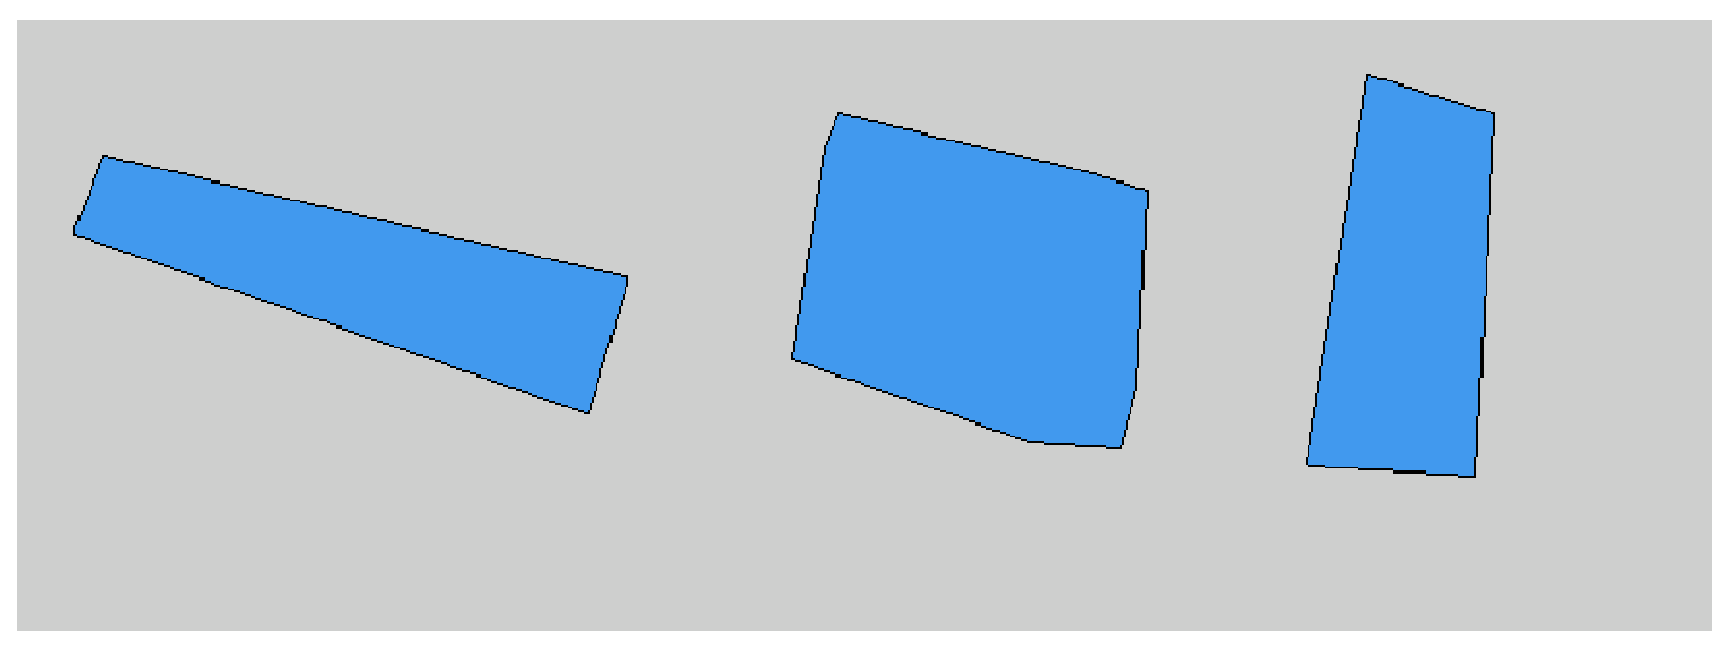
\includegraphics[scale=0.6]{Rotation.eps}
	\caption[Die Schwächen des Verfahrens für große Rotationen]{Ein Beispiel, in dem man die Schwäche des Verfahrens bei großen Rotationen sehen kann.}
	\label{fig:BeispielschlechteRot}
\end{figure}

\subsection{Konvexer Hüllenbaum\index{ConvexHullTreeNode!Konzept}}

Das obige Verfahren kann nur mit konvexen Polygonen umgehen. Um einfache Polygone bearbeiten zu können, führen die Autoren den \textit{ConvexHullTree} ein. Die Idee hinter diesem ist es, einfache Polygone als konvexe Polygone mit konvexen Löchern aufzufassen. 

Ein \textit{ConvexHullTreeNode} ist ein konvexes Polygon, bei dem jeder Kante wiederum ein \textit{ConvexHullTreeNode} zugeordnet werden kann. Diese Kindelemente werden von dem Vaterelement abgezogen. Abbildung~\vref{fig:ConHullTree} zeigt einen solches Konstrukt.

\begin{figure}
	\centering
	
\includegraphics{feu_logo2.eps}
	\caption{Ein Beispiel für einen ConvexHullTree.}
	\label{fig:ConHullTree}
\end{figure}

Die Veröffentlichung beschreibt, wie man einen solchen Baum aufbaut. Dieses Verfahren ist näher unter \vref{constCHTN} beschrieben.

Die Komplexität der Konstruktion eines Hüllenbaumes wird mit $O(dn*\log(n))$ angegeben, wobei $d$ die Tiefe des resultierenden Baumes ist.

Der umgekehrte Weg, also aus einem \textit{ConvexHullTree} wieder ein Polygon zu erzeugen, funktioniert so:

\begin{itemize}
\item Gebe jedes Segment zurück, für das es kein Kindelement gibt.
\item Für jedes Segment, welches ein Kindelement hat, benutze diese Funktion rekursiv.
\end{itemize}

\subsection{Matching zweier Regionen}

Im Weiteren beschäftigen sich die Autoren mit der Frage, wie man zu gegebenen Polygonen, welche die beiden Schnappschüsse einer MovingRegion darstellen sollen, ein \textit{Match} bestimmen kann. Ein \textit{Match} ist eine Menge von Paaren zusammengehörender \textit{Cycles}. Die erste Komponente der einzelenen Paare werden im Folgenden ,,Sourceen''\index{Source}, die zweiten ,,Targets''\index{Target} genannt.

Die Autoren unterscheiden drei verschiedene Arten von \textit{Matches}:

\begin{enumerate}
\item Beide \textit{Regionen} sind aus mehreren \textit{Faces} zusammengesetzt.
 
Welche \textit{Faces} auf der einen Seite passt dann zu welchen \textit{Faces} auf der anderen Seite?
\item Ein \textit{Face} hat mehrere \textit{Holes}.
 
Welches \textit{Hole} auf der einen Seite passt dann zu welchem \textit{Hole} auf der anderen Seite?
\item Ein \textit{Cycle} hat mehrere Konkativitäten.
 
Welche Konkavitäten auf der einen Seite passen zu welchen Konkavitäten auf der anderen Seite?
\end{enumerate}

In all diesen Fällen ist auch noch zu beachten, dass einzelne Objekte verschwinden können oder dass mehrere Objekte auf der einen Seite zu einem Objekt auf der anderen Seite verschmelzen können.

Um die Qualität eines Matches bestimmen zu können, geben die Autoren einige Kriterien an:

\begin{enumerate}
\item Ein Matching-Verfahren sollte das korrekte Ergebnis liefern, falls beide Schnappschüsse übereinstimmen.
\item Komponenten, die sich relativ zu ihrer Größe wenig bewegt haben, sollten korrekt gematcht werden können.
\item Komponenten, die nur kleine Änderungen an Größe und Form erfahren haben, sollten korrekt gematcht werden.
\item Ein Matching-Verfahren sollte Komponenten erkennen, die sich in mehrere neue aufgesplittet haben oder solche, die sich vereinigen.
\item Ein Matching-Verfahren sollte Kriterien anbieten um zu entscheiden, ob zwei Momentaufnahmen gut zueinander passen oder ob der zeitliche Abstand zwischen diesen zu groß gewählt ist.
\end{enumerate}

Die Autoren führen den Begriff des ,,sicheren'' Matches ein:

\par
\begingroup
\leftskip=2em 
Sei $mr$ eine \textit{MovingRegion} und seien $S_1$ und $S_2$ zwei Schnappschüsse dieser \textit{MovingRegion} zu den Zeitpunkten $t$ und $t+\Delta t$. Ein Matching-Verfahren ist sicher zu nennen, falls es ein $\epsilon >0$ gibt, so dass das Match korrekte Ergebnisse liefert, für alle $\Delta t < \epsilon$.
\par
\endgroup

Die Autoren finden drei verschiedene Matching-Strategien, die im Folgenden kurz aufgef"uhrt werden:
\begin{enumerate}
\item Position of centroid \label{MatchSchwer}

Bestimme den Schwerpunkt jedes \textit{Cycles},  bilde aus diesem einen gewichteten Graphen mit den Entfernungen als Kantengewichte und suche in diesem "`n"achste Nachbarn"'.
\item Fixed threshold (set of cycles)\label{fixedThre}

Gegeben sei ein Schwellwert, threshold. Matche zwei \textit{Cycles}, wenn sie sich wechselseitig  mehr als threshold (in \%) überlappen.

\item Maximize Overlap (set of cycles)

Bilde einen gewichteten Graphen, in dem die \textit{Cycles} Knoten sind und dessen Kanten mit dem Grad der Überlappung gewichtet sind. Matche dann ein \textit{Cycle} $c$ mit demjenigen, mit dem er die gr"o"ste Überlappung aufweist und mit allen, f"ur die $c$ der \textit{Cycle} mit der gr"o"sten Überlappung ist.
\end{enumerate} 

Die Autoren kommen zu dem Schluss, dass das Schwerpunktverfahren kein sicheres Verfahren sei, da der Schwerpunkt eines Polygons auch außerhalb liegen kann.

Im weiteren Verlauf betrachten die Autoren nur noch einzelne \textit{Cycles}; Betrachtungen von \textit{Faces} und \textit{Regions} werden nicht mehr angestellt.

\subsection{Interpolation zwischen zwei \textit{ConvexHullTrees}}

Im weiteren beschäftigen sich die Autoren damit, einen Algorithmus zu erarbeiten, mit dessen Hilfe sich eine Interpolation zwischen zwei einfachen Polygonen berechnen läßt. Dieser Algorithmus beruht darauf, den Rotating--Plane--Algorithmus für alle konvexen Hüllen durchlaufen zu lassen und hierbei die Darstellung des Polygons als \textit{ConvexHullTree} zu benutzen.

Gegeben seien  zwei einfache Polygone $A$ und $B$ dargestellt als \textit{ConvexHullTrees}. Das Matching zwischen diesen sei so berechnet, dass man für alle Elemente von $A$ bestimmen kann, welche Elemente von $B$ dazu passen.

Wir nehmen an, dass $A$ auf $B$ gematcht wird, und berechnen für die konvexen Hüllen von $A$ und $B$ die \textit{MovingSegments} mit dem  Rotating--Plane. 

Nehmen wir nun an, dass eine Konkavität von $A$ keiner Konkavität von $B$ zugeordnet wird. Abbildung~\vref{fig:Interpolationnonconvex} zeigt ein solches Beispiel. Die Punkte, an denen diese Konkavität die konvexe Hülle des Vaters berührt, nennen wir $p$ und $e$. In diesem Fall bestimmen wir das \textit{MovingSegment} aus den bereits Berechneten, das $p$ und $e$ enthält. Dieses \textit{MovingSegment}, dessen dritten Punkt wir $t$ nennen, löschen wir. Falls dieses MSegement kein Dreieck ist,dann muss es ein Viereck sein, so dass wir dieses zuerst in zwei Dreiecke spalten. Nun bilden wir für alle Kanten der konvexen Hülle der Konkavität, außer $\bar{pe}$, \textit{MovingSegmente} mit dem Punkt $t$ und fügen diese dem Ergebnis hinzu.

Wird eine Konkavität von $A$ gegen eine Konkavität von $B$ gematcht, so bilden wir mittels Rotating-Plane, die \textit{MovingSegmente} zwischen diesen und fügen sie der Ergebnisliste an. In dieser Liste werden jetzt zwei oder vier paarweise gleiche \textit{MovingSegmente} vorkommen\footnote{Bei der praktischen Anwendung dieses Algorithmuss zeigte sich, dass dies durchaus nicht immer der Fall ist (siehe~\vref{gedrehtKon}).}. Diese Segmente, die die Schnittstelle zwischen der Vater und der konvexen Hülle des Kindes bilden, werden gelöscht. 

Der dritte, komplizierteste Fall tritt auf, wenn mehrere Konkavitäten auf der einen Seite zu einer auf der anderen Seite verschmelzen. Für diesen Fall erarbeiten die Autoren einen Algorithmus der darauf beruht, von mehreren Konkavitäten die konvexe Hülle zu berechnen und diese auf die eine Konkativität der anderen Seite zu matchen. Damit das Verfahren danach weiterlaufen kann, wird der ConvexHullTree auf der mehrdeutigen Seite umgebaut, so dass die Kinder der Konkavitäten geeignet an die neue konvexe Hülle gehängt werden\footnote{Leider funktioniert dieses Verfahren nicht in allen Fällen (siehe~\vref{JoinConc}).}.

\begin{figure}
	\centering
	
\includegraphics{feu_logo2.eps}
	\caption{Interpolation zwischen nicht konvexen Polygonen.}
	\label{fig:Interpolationnonconvex}
\end{figure}

\subsection{Bedeutung für die vorliegende Arbeit}

Die zitierte Veröffentlichung war der Ausgangspunkt dieser Arbeit und ist als solcher von zentraler Bedeutung.

Die Java-Applikation, die im Rahmen des Papers vorgestellt wurde, wurde in der vorliegenden Arbeit in einem ersten Arbeitsschritt ausgebaut, so dass diese auch mit \textit{Regionen}, bestehend aus mehreren \textit{Faces} und mit \textit{Löchern} umgehen kann. In einem nächsten Schritt wurde diese neue Applikation dann in das SECONDO-System integriert.

An dieser Stelle soll der Begriff des \textit{RegionTrees} definiert werden, da er zum Verständnis der weiteren Arbeit unerlässlich ist. Der \textit{RegionTree} ist eine Erweiterung des \textit{ConvexHullTrees}, so dass dieser ganze Regionen abbilden kann. 

\index{RegionTree}Ein \textit{RegionTree} besteht aus einem oder mehreren \textit{Faces} als \textit{RegionTreeNodes}. Ein \textit{Face} als \textit{RegionTreeNode} besteht aus einem \textit{Cycle} und einer Menge von \textit{Holes}, die alle durch \textit{ConvexHullTrees} dargestellt werden. Abbildung~\vref{fig:RegionTreeNode} zeigt den Aufbau dieses Baumes. \textit{Regions}, \textit{Faces} und \textit{ConvexHullTreeNodes} werdem im Folgenden als \textit{RegionTreeNodes} bezeichnet.

\begin{figure}
	\centering
	
\includegraphics{feu_logo2.eps}
	\caption{Der strukturelle Aufbau eines RegionTrees}
	\label{fig:RegionTreeNode}
\end{figure}

\section[Matching Shapes with a Reference Point]{Das Paper: ,,Matching Shapes with a Reference Point'' }\label{AARR}

Als eine sehr interessante Quelle erwies sich das Paper \cite{AAR}, dessen Inhalt hier kurz zusammengefasst werden soll.

\subsection{Metrik und Ähnlichkeit}

In ihrer Arbeit betrachten die Autoren Ähnlichkeiten von Objekten, die als Punktmengen repräsentiert werden. Diese Betrachtungen haben besondere Relevanz in Anwendungen der Mustererkennung. Als Maß für die Ähnlichkeit von zwei Objekten wird hier wie auch in den meisten anderen Arbeiten zu diesen Themen der Hausdorff--Abstand\index{Hausdorff--Abstand!als Norm} benutzt, der unter \vref{Hausdorff} näher beschrieben wird.

Um die Ähnlichkeit  zweier Objekte $A$ und $B$ aus $\mathbb{R}^2$ oder aus $\mathbb{R}^3$ zu bestimmen, reicht es nicht, den Hausdorff-Abstand $\delta_H(A,B)$ zu bestimmen, sondern man sucht die Abbildung $T\in\mathcal{T}$ unter der $\delta_H(A,T(B))$ minimal ist. $\mathcal{T}$ ist hierbei die Menge aller ,,erlaubten'' Abbildungen. Solche Abbildungen sind üblicherweise Rotationen, Verschiebungen, Skalierungen und Kombinationen aus solchen. Also sucht man:

$$\min_{T\in\mathcal{T}}\delta_H(A,T(B))$$

Die Suche nach dem optimalen $T$ kann im Allgemeinen sehr kompliziert und aufwändig. Deshalb versuchen die Autoren keine optimale Abbildung $T_{OPT}$ zu finden, sondern sie suchen nach einer einfach und schnell berechenbaren Näherung, also einer Abbildung $T_{Approx}$, die $T_{OPT}$ zuverlässig und hinreichend gut annähert.

\subsection{\index{Match!pseudo--optimales}Pseudo--optimales Match}

Die Autoren definieren eine Abbildung als ,,pseudo--optimales Match mit Fehlerfaktor $\alpha$''  ($\alpha\geq 1$, $\delta$ ist der optimale Hausdorff--Abstand), falls gilt:

$$\delta_H(A,T(B))\leq \alpha \delta$$

\subsection{\index{Referenzpunkt!Definition}Definition des Refenenzpunktes}

Den Versuch ein solches pseudo--optimales Matching zu finden, unternehmen die Autoren über Referenzpunkte. Als Referenzpunkt im Bezug auf $\mathcal{T}$ definieren sie eine Abbildung $s:C^d\longrightarrow\mathbb{R}^d$, für die gilt:
$$\forall A, B\in C^d  \:\wedge\: \forall\: T\in\mathcal{T}\Rightarrow$$
$$s(T(A))=T(s(A))\text{ (s ist äquivariant) und}$$
$$\exists c\geq0 \: :\: \forall A, B \in C^d\Rightarrow$$
$$\Vert s(A)-s(B)\Vert\leq c\cdot\delta_H(A,B)\text{ (s ist Lipschitz--stetig mit Konstante c)}.$$

Die Autoren nennen $c$ auch die Qualität von $s$.

\subsection{Algorithmen zum Finden pseudo--optimaler Lösungen}

Unter der Annahme, dass ein geeigneter Referenzpunkt gefunden wurde, entwickeln die Autoren drei Algorithmen:
\begin{itemize}
\item Algorithmus $T$
\begin{enumerate}
\item Berechne $s(A)$ und $s(B)$.
\item Die pseudo--optimale Lösung ist die Verschiebung um den Vektor $s(A)-s(B)$. Das Bild von $B$ nenne $B'$.
\end{enumerate}

\item Algorithmus $R$
\begin{enumerate}
\item Wie in $T$.
\item Finde die optimale Rotation von $B'$ um $s(A)$. Diese Rotation, verknüpft mit der Verschiebung aus $T$, ist die pseudo--optimale Lösung. Das Bild dieser nenne im Weiteren $B''$.

\end{enumerate}
\item Algorithmus $S$
\begin{enumerate}
\item Wie in $R$.
\item Bestimme die Durchmesser $d(A)$ und $d(B)$ und skaliere $B'$ um den Faktor $\alpha =\frac{d(A)}{d(B)}$.
\item Wie Schritt 2 in $R$.
\end{enumerate}
\end{itemize}

Dann beweisen die Autoren:
\begin{enumerate}
\item Algorithmus $T$ findet eine pseudo--optimale Abbildung für Verschiebungen. Der Fehlerfaktor ist $\alpha=c+1$.
\item Algorithmus $R$ findet eine pseudo--optimale Abbildung für Kompositionen aus Verschiebungen und Rotationen.  Der Verlustfaktor ist $\alpha=c+1$.
\item Algorithmus $S$ findet eine pseudo--optimale Abbildung für Kompositionen aus Verschiebungen, Rotationen und Skalierungen. Der Verlustfaktor ist $\alpha=c+3$.
\end{enumerate}

\subsection{\index{Referenzpunkt!Steiner--Punkt}\index{Steiner--Punkt!als Referenzpunkt}Wahl des richtigen Referenzpunktes}

Im weiteren Verlauf werden verschiedene Referenzpunkte untersucht. Der Schwerpunkt der konvexen Hüllen der Polygone ist ein Referenzpunkt mit der Qualität $c=4\pi+3$. Der beste Referenzpunkt, den die Autoren finden konnten, ist der Steiner--Punkt, der in \vref{Steinerpunkt} beschrieben wird. Die Autoren zeigen, dass der Steiner--Punkt ein Referenzpunkt für alle untersuchten Abbildungen ist und zeigen, dass dessen Qualität im zweidimensionalen $c=\frac{4}{\pi}$ ist. 

\subsection{Untere Schranke für die Qualitäten von Referenzpunkten}

Zuletzt finden die Autoren eine untere Schranke für die Qualität eines zweidimensionalen Referenzpunktes, unter Verschiebungen. Die Qualität eines Referenzpunktes unter diesen Abbildungen kann nicht besser sein als $\sqrt{\frac{4}{3}}$. Diese Behauptung wird bewiesen. 

Vergleicht man die Qualität des Steiner--Punktes ($\frac{4}{\pi}\thickapprox 1,155$) mit diesem theoretischen minimalen Wert ($\sqrt{\frac{4}{3}}\thickapprox 1,27$) stellt man fest, dass der Abstand der Qualitäten sehr gering ist. Der Steiner--Punkt ist also wahrscheinlich der beste mögliche Referenzpunkt (für die Norm ,,Hausdorff--Abstand'').

\subsection{Bedeutung für diese Arbeit}\label{BedeutungAAR}

Zwar habe wurde dieses Matching nicht so implementiert, wie es hier beschrieben wird, stattdessen wurde aber ein Match programmiert das simultan zu dem Schwerpunkt-Match mit Schwellenwert von Erlend T\o{}ssebro (siehe \vref{MatchSchwer}) funktioniert, nur dass hierbei der Schwerpunkt durch der Steinerpunkt ersetzt wird.

Betrachtet man den T\o{}ssebro'schen Algorithmus, so stellt man fest, dass dieser starke Ähnlichkeit zu dem Algorithmus $T$ aus diesem Paper aufweist. Es steht also zu erwarten, dass dieser Algorithmus Matches finden wird, die gute Ergebnisse bezüglich des Hausdorff-Abstands liefern werden. Die hier beschriebenen Algorithmen konkret umzusetzen wäre zwar sinnvoll, überschreitet aber den Umfang dieser Arbeit.

\section[Matching Shapes with Symmetric Difference]{Das Paper: ,,Matching Convex Shapes with Respect to Symmetric Difference'' }\label{AFRWW}

Als eine weitere sehr interessante Quelle erwies sich die Arbeit \cite{AFRW}, die stark auf der anderen aufbaut. 

\subsection{Grundlagen}

Zunächst klären die Autoren die Grundlagen dieser Arbeit. Da dieses Paper auf \cite{AAR} aufbaut, sind diese Grundlagen bereits aus dieser Arbeit bekannt. 

\subsection{\index{symmetrische Differenz!als Norm}Die symmetrische Differenz als Norm}

Als neue Norm für die Ähnlichkeit zweier Objekte wird die symmetrische Differenz beschrieben. Diese ist unter  \vref{symDiff} näher beschrieben. Die Autoren machen darauf aufmerksam, dass diese Norm ein ,,gutmütigeres'' Verhalten an den Tag legt, wenn die zu matchenden Polygone ,,gestört'' sind. Gestört soll in diesem Zusammenhang heißen, dass an sich an dem Rand des eigentlichen Polygons schmale, lange Dreiecke befinden. Unter \vref{symDiff} wird auch dieser Zusammenhang näher erläutert.

\subsection{\index{Schwerpunkt!als Referenzpunkt}\index{Referenzpunkt!Schwerpunkt}Der Schwerpunkt als Referenzpunkt für Verschiebungen}

Als Referenzpunkt für Abbildungen unter dieser Norm wird der Schwerpunkt der Polygone betrachtet. Dieser wird in dem Paper  nicht näher erläutert, er wird hiertrotzdem unter \vref{Schwerp} beschrieben. 

Für $A, B \in \mathbb{R}^2$ und  die Menge der Verschiebungen $\mathcal{T}$ wird der Satz

$$\delta_C (A,V(B))\leq\frac{11}{3}\min_{T\in\mathcal{T}}\delta_C(A,T(B))$$


aufgestellt und bewiesen. $V$ ist hierbei diejenige Translation, die den Schwerpunkt von $B$ auf den Schwerpunkt von $A$ verschiebt.

\subsection{Allgemeinere Abbildungen}

Um diesen Referenzpunkt auch auf andere Abbildungen anwenden zu können, wird folgender Satz aufgestellt und bewiesen:

\par
\begingroup
\leftskip=2em 

Gilt für eine Menge $\mathcal{T}$  von Abbildungen 
\begin{enumerate}
\item $s(T(A))=T(s(B))$ für $T\in\mathcal{T}$ und 
\item $\mathcal{T}$ ist abgeschlossen bezüglich der Komposition von Abbildungen.
\end{enumerate}
dann ist der Schwerpunkt ein  Referenzpunkt mit Qualität $\frac{11}{3}$, bezogen auf $\mathcal{T}$.
\par
\endgroup
Abbildungen, die diese Bedingung erfüllen sind: 
\begin{itemize}
\item Kombinationen aus Verschiebungen und Rotationen,
\item Kombinationen aus Verschiebungen und Skalierungen,
\item Kombinationen aus allen drei Abbildungsarten und
\item beliebige affine Abbildungen.
\end{itemize}

\subsection{Algorithmen zum Finden von pseudo--optimalen Lösungen}

Nun erarbeiten die Autoren verschiedene Algorithmen, um Matchings für die verschiedenen Abbildungsarten durchführen zu können:
\begin{enumerate}
\item Verschiebungen

Verschiebt man $B$ um den Vektor $s(B)-s(A)$ auf $B'$, so hat man ein pseudo--optimales Matching gefunden. Dieser Algorithmus entspricht dem Algorithmus $T$ aus dem letzten Abschnitt.

\item Kombinationen von Verschiebungen und Skalierungen

Verschiebt man zunächst $B$ wie oben angegeben und skaliert dann $B'$ bezogen auf den Fixpunkt $s(A)$ um den Faktor $\lambda$, so hat man ein pseudo--optimales Matching gefunden. $\lambda$ ist hierbei der Faktor, bei dem $\delta_C(A,\lambda B')$ minimal ist. Dieser Faktor kann in Linearzeit berechnet werden, wie die Autoren zeigen.

\item Kombinationen aus Verschiebungen und Drehungen

Auch hier wird zunächst $B'$ durch Verschiebung, wie oben, gebildet. Nun wird der Winkel $\varphi$ gesucht, für den $\delta_C(A,t_\varphi( B'))$ minimal ist. $t_\varphi$ sei die Rotations-Abbildung um den Punkt $s(A)$. Eine wirklich effiziente Lösung dieses Problems können die Autoren leider nicht geben, so dass man noch keinen effizienten Algorithmus für Abbildungen angeben kann, die Rotationen enthalten. 
\end{enumerate}

\subsection{Fazit}

Falls man die symmetrische Differenz als Norm benutzt, kann man  zusammenfassend sagen:
\begin{itemize}
\item Schwerpunkte sind Referenzpunkte für alle relevanten Abbildungen und
\item das Matching auf dieser Grundlage für alle Kombinationen aus Verschiebungen und Skalierungen ein pseudooptimales Matching mit der Qualität $\frac{11}{3}$ liefert. 
\end{itemize} 
\subsection{Bedeutung für diese Arbeit}\label{BedeutungAFRW}

Ein Matching, welches den Schwerpunkt als Referenzpunkt benutzt hat, ist ebenso bereits in der Arbeit von T\o{}ssebro enthalten (siehe~\vref{MatchSchwer}), wie auch ein Matching, das die Überlappung, also das Inverse der symmetrischen Differenz, benutzt. Zwar sind dessen Algorithmen, wie auch bei der vorhergegangenen Arbeit, nicht so ausgefeilt wie die Algorithmen dieses Papers, aber nach der Lektüre dieser Arbeit läßt sich vermuten, dass die Resultate des Schwerpunkt-Matchings und die des Überlappungs-Matchings starke Ähnlichkeiten aufweisen werden. 

\section{Grundlagen der Paper}
In den oben beschriebenen Papern wurden einige wichtige, allgemeingültige Begriffe eingeführt. Die Definition dieser wichtigen Begriffe sollen im folgenden Abschnitt kompakt zusammengefasst werden.

\subsection{\index{Hausdorff--Abstand!Definition und Berechnung}Hausdorff--Abstand}\label{Hausdorff} 

Seien $A$ und $B$ zwei kompakte Teilmengen des $\mathbb{R}^2$ und sei $\Vert\centerdot\Vert$ die Euklidische Norm.
Dann definieren wir eine Hilfsfunktion $ \widetilde{\delta_H}  $, den einseitigen Hausdorff--Abstand, wie folgt:
\[ \widetilde{\delta_H}(A,B):=\max_{a\in A} \;\min_{b\in B} \Vert a-b \Vert\]
Der einseitige Hausdorff-Abstand von Polygon $A$ zu Polygon $B$ ist so definiert, dass er der Abstand des am weitesten entfernten Punktes aus $A$ zu dem ihm am n"achsten gelegenen Punkt aus $B$ ist.  Im weiteren Schritt wird der Hausdorff--Abstand wie folgt definiert: 
\[\delta_H:=\max\{\widetilde{\delta_H}(A,B),\widetilde{\delta_H}(B,A)\}.\]
\begin{figure}
	\centering
	\includegraphics[scale=.6]{Hausdorff.eps}
	\caption[Der Hausdorff--Abstand zweier Polygone]{Der Hausdorff--Abstand zweier Polygone (grün und blau) ist das Paar mit dem größten Abstand (rot) unter allen Paaren.}
	\label{fig:HausdorffAbstand}
\end{figure}
Nimmt man also von zwei Polygonen zu jedem Punkt der einen Menge den nächsten Punkt der anderen Menge (und umgekehrt) und sucht dann das Paar mit dem größten Abstand, so ist dieser der Hausdorff--Abstand. Abbildung~\vref{fig:HausdorffAbstand} zeigt das beispielhaft.



\subsection{\index{symmetrische Differenz!Definition}Die symmetrische Differenz}\label{symDiff}
\begin{figure}
	\centering
	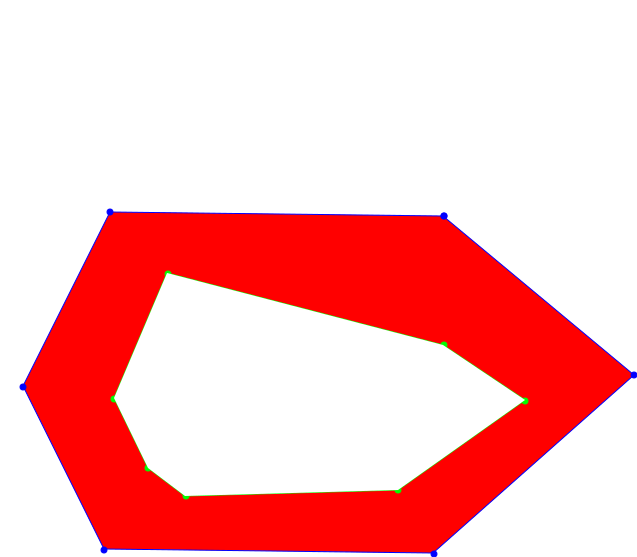
\includegraphics[scale=.6]{SymDiff.eps}
	\caption[Die symmetrische Differenz zweier Polygone]{Die symmetrische Differenz der beiden Polygone aus dem Schaubild~\vref{fig:HausdorffAbstand} ist der Flächeninhalt der roten Fläche.}
	\label{fig:SymDiffBild}
\end{figure}

In \cite{AFRW} wird vorgeschlagen, den Fl"acheninhalt der symmetrischen Differenz als Abstands-Ma"s zweier konvexer Polygone zu benutzen. Die symmetrische Differenz von zwei kompakten Teilmengen $A$ und $B$ des $\mathbb{R}^2 $ ist definiert als:
\[A\bigtriangleup B:=(A\setminus B)\cup(B\setminus A).\]
Wenn $\Vert\cdot\Vert$ der Fl"acheninhalt ist, so bildet $\delta_S$ den Abstand nach der symmetrischen Differenz:
\[\delta_S:=\Vert A \bigtriangleup B\Vert.\]
In \cite{TG} schlagen die Autoren vor, die Überlappung $A\cap B$ als Maß für die Qualität eines Matchings zu benutzen. Wegen:
$$|A\bigtriangleup B|+|A\cap B|=|A\cup B|$$
ist ersichtlich, dass ein Match, welches die symmetrische Differenz minimiert, zu dem selben Ergebnis kommen wird wie ein Match, das die Überlappung maximiert.

In \cite{AFRW} wurde beschrieben, dass das Verhalten der symmetrischen Differenz relativ ,,gutmütig'' im Bezug auf gestörte Daten ist. Die Zeichnung~\vref{fig:VergleichMetrik} illustriert diesen Zusammenhang. Die beiden Polygone sehen den Polygonen aus den Bildern~\vref{fig:HausdorffAbstand} und \vref{fig:SymDiffBild} recht ähnlich, nur zwei Punkte sind in jedem Polygon ergänzt worden. Dennoch ist der Hausdorff--Abstand um 100\% gestiegen, die Fläche der symmetrischen Differenz hingegen nur etwa um 8\%.

\begin{figure}
	\centering
	\includegraphics[scale=.6]{Metrikengestoert.eps}
	\caption{Hausdorff-Abstand und symmetrische Differenz im Vergleich}
	\label{fig:VergleichMetrik}
\end{figure}


\subsection{\index{Steiner--Punkt!Definition}Der Steiner--Punkt}\label{Steinerpunkt}

In \cite{Sch} wird der Steiner--Punkt beschrieben \textit{"`als Schwerpunkt der Massenverteilung, die bei einem konvexen Polygon durch Belegung der Ecken mit den "au"seren Winkeln als Massen [...] gegeben ist"'}. Folglich kann der Steiner--Punkt eines konvexen Polygons $P$, das aus den $n$ Eckpunkten $v_i$ besteht, berechnet werden ($\alpha_i$ ist hierbei der Innenwinkel von $v_i$) durch:
\[p_2(P)=\sum^n_{i=1}v_i (\pi-\alpha_i).\]
In der Zeichnung~\vref{fig:Referenzpunkte} ist der Steiner-Punkt grün eingezeichnet.


\subsection{\index{Schwerpunkt!Definition}Der Schwerpunkt}\label{Schwerp}

Der Schwerpunkt eines Polygons ist der Schwerpunkt der Massenverteilung, die entsteht, wenn man allen Eckpunkten die gleiche Masse zuordnet. Er berechnet sich f"ur ein Polygon $P$ mit $n$ Eckpunkten $v_i$:
\[p_0(P)=\sum^n_{i=1}v_i \frac{1}{n}.\]
In der Zeichnung~\vref{fig:Referenzpunkte} ist der Schwerpunkt rot markiert. 

Vergleicht man die beiden Referenzpunkte, so kann man sehen, dass der Schwerpunkt etwas ,,träger'' auf Punkte reagiert, die sich stark von den anderen unterscheiden (in dem dargestellten Beispiel der Punkt ganz rechts). In einem regelmäßigen n"~Eck stimmen entsprechend beide Referenzpunkte überein. Vergleicht man dieses Verhalten der Referenzpunkte mit dem Verhalten der Normen für gestörte Werte (siehe Abbildung \vref{fig:VergleichMetrik}), so erscheint der Zusammenhang vom ,,empfindlicheren'' Hausdorff--Abstand und dem  Steiner--Punkt, sowie der Zusammenhang zwischen den beiden ,,Gutmütigeren'' plausibel.

\begin{figure}
	\centering
	\includegraphics[scale=.8]{Referenzpunkte.eps}
	\caption[Vergleich beider Referenzpunkte]{Hier kann man beide Referenzpunkte im Vergleich sehen (der Schwerpunkt der Massenverteilung ist rot, der Steinerpunkt grün) }
	\label{fig:Referenzpunkte}
\end{figure}


